\documentclass{ifacconf}

\usepackage{natbib}            % you should have natbib.sty
\usepackage{graphicx}          % Include this line if your 
\usepackage{todo}
\usepackage{subfigure}
\usepackage{hyperref}
\usepackage{breakurl}

                               % document contains figures,
%\usepackage[dvips]{epsfig}    % or this line, depending on which
                               % you prefer.													
% predefined environments
%\begin{thm} ... \end{thm}		% Theorem
%\begin{lem} ... \end{lem}		% Lemma
%\begin{claim} ... \end{claim}	% Claim
%\begin{conj} ... \end{conj}	% Conjecture
%\begin{cor} ... \end{cor}		% Corollary
%\begin{fact} ... \end{fact}	% Fact
%\begin{hypo} ... \end{hypo}	% Hypothesis
%\begin{prop} ... \end{prop}	% Proposition
%\begin{crit} ... \end{crit}	% Criterion

\begin{document}

\begin{frontmatter}

\title{Scaling Communication of flexibility Object in Many-to-one using Distributed Aggregation} % Title, preferably not more than 10 words.

\thanks[footnoteinfo]{This article is written as a part of the course Publishing Papers in the Peer-Reviewing System. It is based on \cite{SCEDFDA} which is authored by Alex B. Andersen, Rasmus V. Prentow, and myself.}

\author[First]{Kim A. Jakobsen} 


\address[First]{Department of Computer Science, Aalborg University, Selma Lagerl\"{o}fs Vej 300 DK-9220 Aalborg East (e-mail: kjakob09@student.aau.dk).}                                              


\begin{abstract}                          
The system MIRABEL allows producers and consumers (prosumers) to offer the balance responsible party (BRP) flexibility. 
This enables the BRP to shift energy demand to when renewable energy is available. 
When the number of flexibility offers (flex-offers) increase it poses a scalability problem. 
The flex-offers can be aggregated into fewer aggregated flex-offers, by creating an intermediate node that preforms aggregation, the number of flex-offers sent to the BRP is reduced.
We define a systematic way to compare strategies and suggest a strategy we call Evenly Distributing Strategy. 
We find the balance between the number of aggregator nodes and flex-offers send to achieve the lowest message load. 
\end{abstract}

\end{frontmatter}

\section{Introduction}
Renewable energy sources such as solar and wind share the undesirable attribute that they are uncontrollable. 
This is in contrast to e.g. fossil-fueled power plants where it is possible to adjust power production according to the energy demand. 
Micro-Request-Based Aggregation, Forecasting and Scheduling of Energy Demand, Supply and Distribution~\cite{mirabel} (MIRABEL) is a EU project that works to allow better utilization of renewable energy. 
Instead of controlling the power production the goal is to predict and control the power consumption. 
If the Balance Responsible Party (BRP) can control when consumers use power and can forecast when renewable energy is produced then it is only necessary to relay on fossil-fuel when renewable energy is sparse.
The MIRABEL system allows consumers and producers (prosumers) of energy to sent an offer of flexibility to the BRP, this is called a flex-offer. 
The BRP is now able to shift when energy is consumed to when renewable energy is produced.


An example of a flex-offer could be the heating of a swimming pool. 
The consumer want his pool heated to 27$^\circ$ Celsius the next morning at 0700AM.
The swimming pool heater sends a flex-offer to the local BRP containing the relevant information such as energy required and the timespan in which the heating can commence.
When the BRP receive the flex-offer it is aggregated with other similar flex-offers. 
The aggregated flex-offer which now corresponds to a larger energy amount can now be shifted to when there are renewable energy available, this is also done by the BRP.  
The pool heater is informed when it should run and the consumer revives a discount on the energy price, as compensation for the offer of flexibility. 


MIRABEL have a large codebase which functions at a proof of concept level, one of the shortcomings in the project is the expensive communication.
The system simulates prosumers which sent flex-offers to a simulated BRP. 
This means that there is a many to one relationship between the prosumers and the BRP, this can be seen in Figure~\ref{fig:prosumerBrp}.
From now on we view the prosumers and the BRP as nodes in the system.
By introducing new intermediate nodes that receive flex-offers from the prosumer, aggregates them, and send the aggregated flex-offers to the BRP node, we can reduce the message load on the BRP node. 
This new node type is called an aggregator node, the new message flow can be seen in Figure~\ref{fig:prosumer-agg-brp}.

\begin{figure*}[]
   \centering
    \subfigure[Without aggregator nodes.]{
    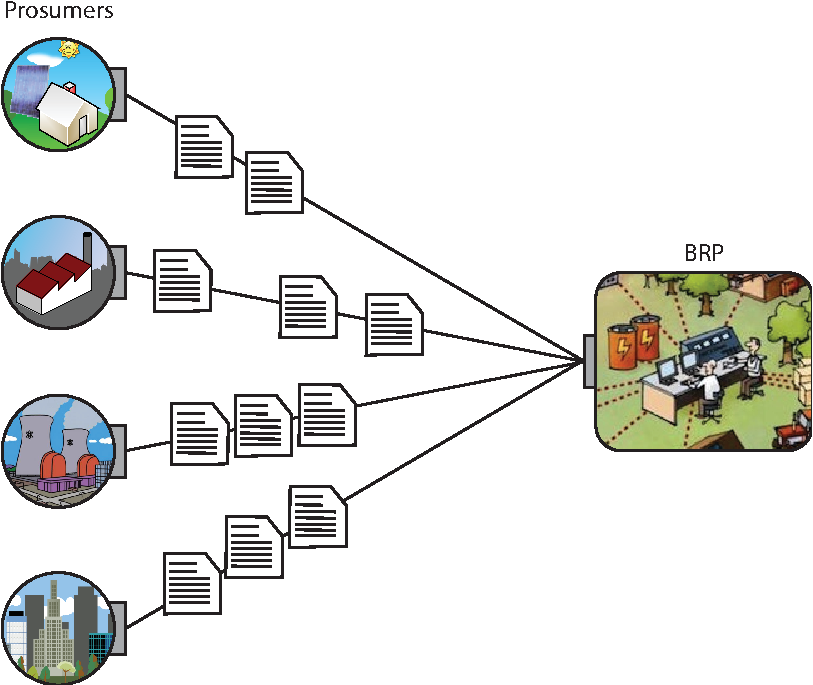
\includegraphics[width=0.75\columnwidth]{images/prosumer-brp.pdf}
    \label{fig:prosumerBrp}
   }
   \subfigure[With aggregator nodes.]{
    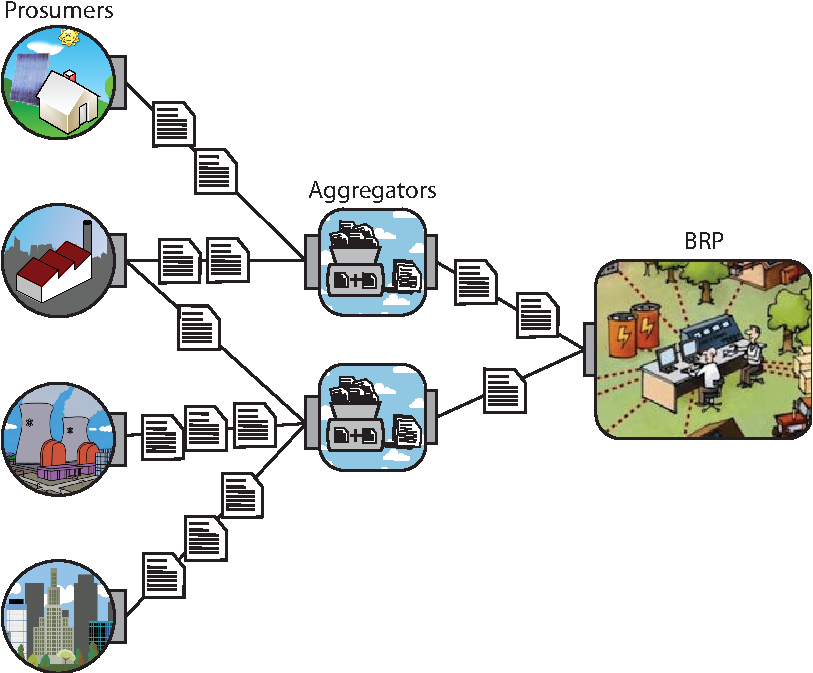
\includegraphics[width=0.75\columnwidth]{images/prosumer-agg-brp.pdf}
    \label{fig:prosumer-agg-brp}
   }  
  \caption{Four prosumers, displayed to the left of each sub-figure, sending flex-offers to a single BRP, displayed to the right.}
  \label{fig:communicationservice}
\end{figure*}


%nodes in mirabel
%report of what happens in the rest of the document

\section{related work}

In \cite{carmeli} they experiment with the position of the aggregation node. 
They do aggregation on sending side, network switches, and intermediate message servers.
The message server set-up is similar to our approach but they assume that all messages can be aggregated which is in contrast to this case.

Aggregation of flex-object which is a generalization of flex-offers, is explored and efficient algorithm are proposed in \cite{ssdbm}. 
These algorithm are implemented in the existing MIRABEL aggregation mechanics which we reuse.

\section{Aggregator Node}

We now know that there is a number of prosumers that sent flex-offers to aggregator nodes. 
The flex-offers are aggregated into fewer aggregated flex-offers and send to the BRP node.
To make it possible to compare different set-ups we define define a strategy.

Formally we describe a strategy as consisting of four elements:
\begin{itemize}
	\item An aggregation function.
	\item A distribution function. 
	\item A set of aggregator nodes.
	\item A BRP node.
\end{itemize} 

An aggregation function it defines how the possible merging of flex-offers is done.
A distribution function defines how the flex-offers is allocated to the different aggregator nodes.
The naive approach is to make a strategy is to use only one aggregator node. 
This aggregator node receives all flex-offers and therefore have the best conditions for aggregating the flex-offers into as few as possible aggregated flex-offers. 
This courses the number of flex-offers sent to the BRP node to be as low as possible. 
However, this would only move the scalability problem to the aggregator node instead of the BRP node. 

To express the desired effects of a strategy we define the measure load.
Load on a given node is defined by the number of flex-offers it receives.
It is desirable to have a strategy that renders as low as possible load on the BRP node and the maximum load of the set of aggregator nodes is low as possible.  


We propose the Evenly Distributing Strategy.
This strategy is defined as following:
\begin{itemize}
	\item As aggregation function we use the proposed algorithm described in \cite{ssdbm}.
	\item As distribution function we use a round-robin algorithm which distribute the flex-offers evenly amongst all the aggregator nodes.
	\item We vary the number of aggregator nodes for different experiments.
	\item A BRP node is used.
\end{itemize}

\section{Experimental Evaluation}
\subsection{Experimental Data}

The data used in this experiment is from~\cite{meregio}. 
We only use consumption data in this experiment because we deem that it is not necessary generate production flex-offers to achieve realistic data.  
All the tests are run in accelerated time.


We test six strategies that only vary on the set of aggregator nodes. The test is conducted with 0, 1, 2, 4, 8, and 16 aggregator nodes. 
To test if the aggregator node reduces the amount of flex-offers received by the BRP node we run the experiment with an average of 100, 1000, and 10,000 flex-offers send per time unit. 

\subsection{Results}

\begin{figure*}[]
   \centering
    \subfigure[Load on the BRP node.]{
    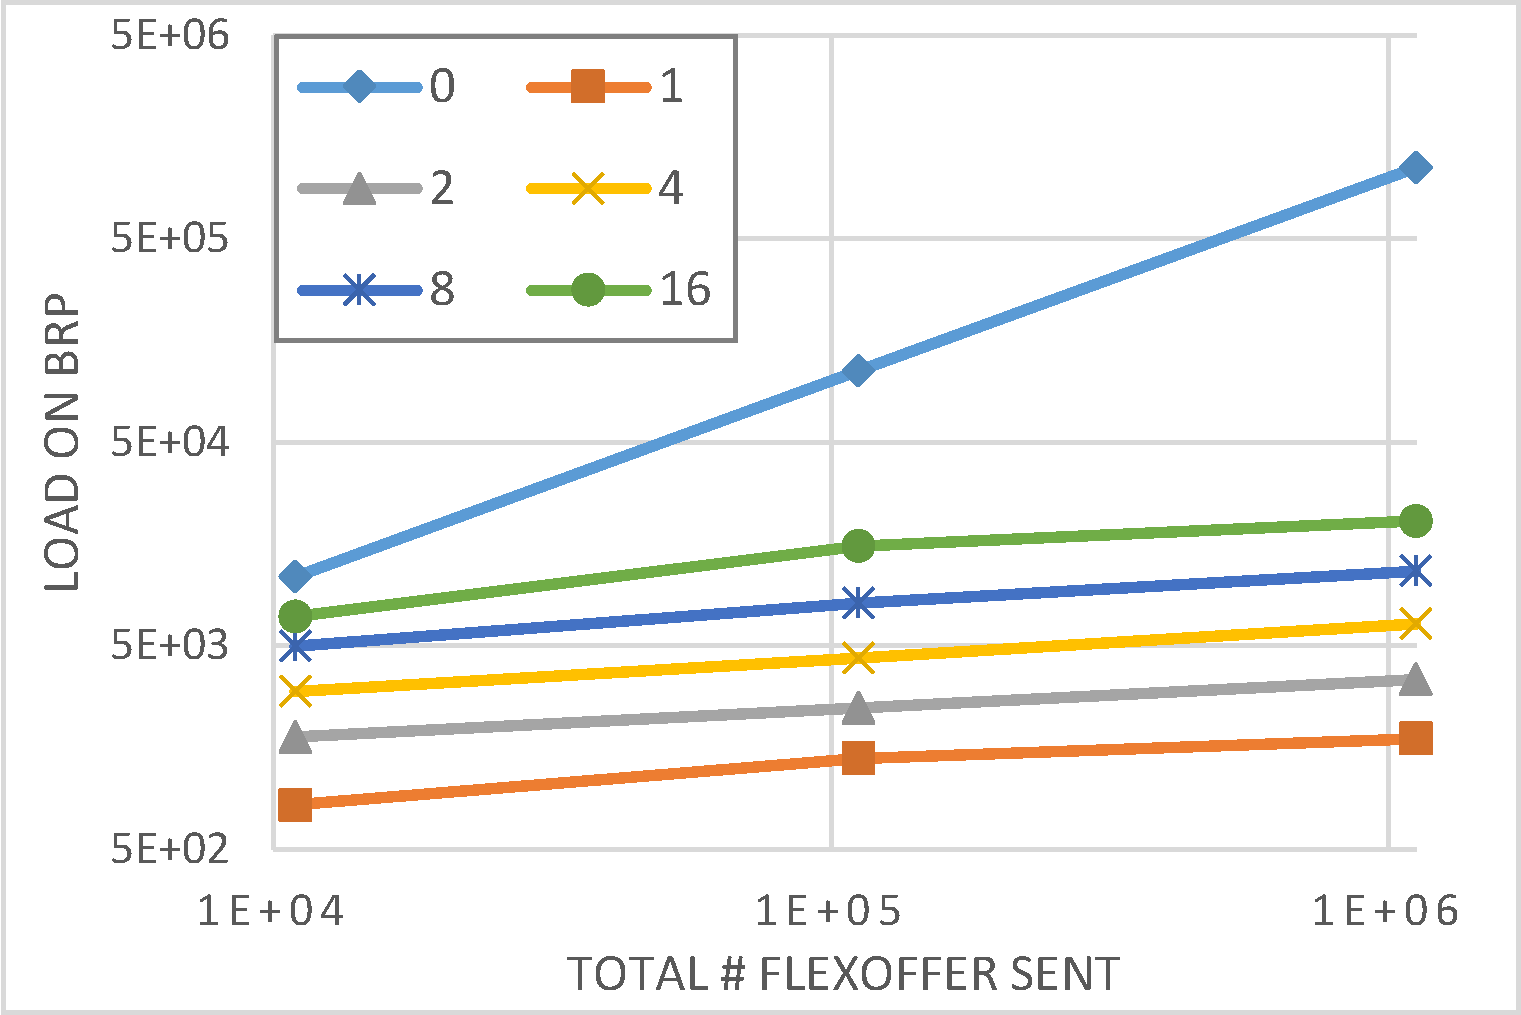
\includegraphics[width=0.75\columnwidth]{images/resultA.pdf}
    \label{fig:resultA}
   }
   \subfigure[Maximum load on the set of Aggregator nodes]{
    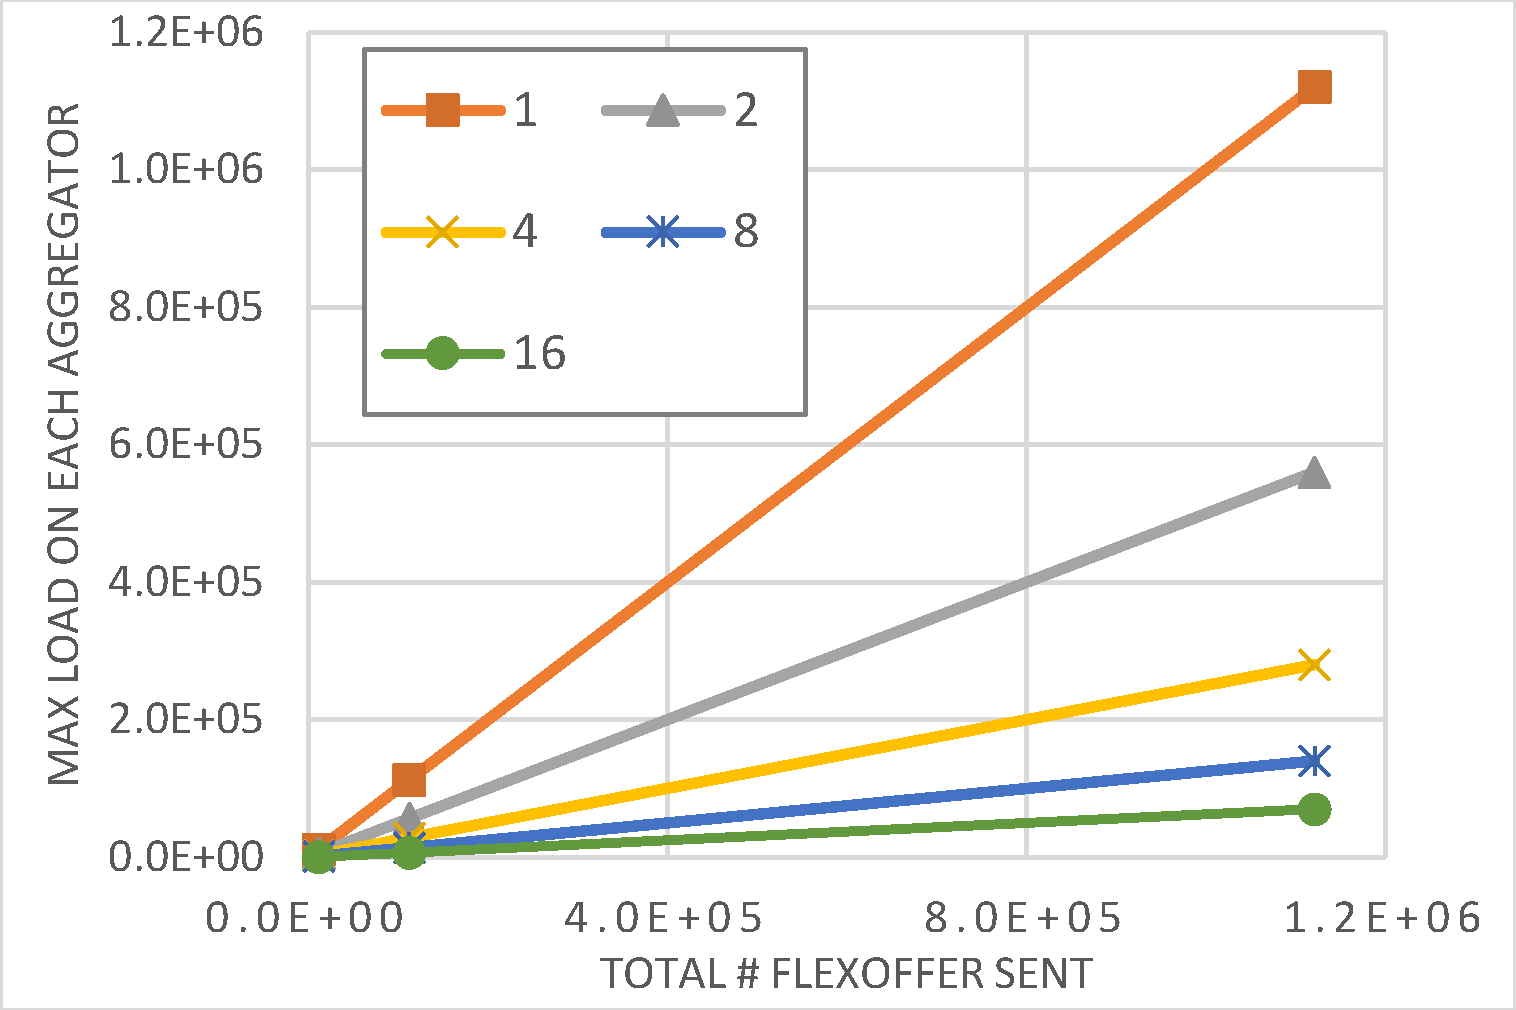
\includegraphics[width=0.75\columnwidth]{images/resultC.pdf}
    \label{fig:resultB}
   }  
  \caption{Test results of different strategies with different amount of flex-offers send per time unit.}
  \label{fig:communicationservice}
\end{figure*}

\begin{figure}%
\centering
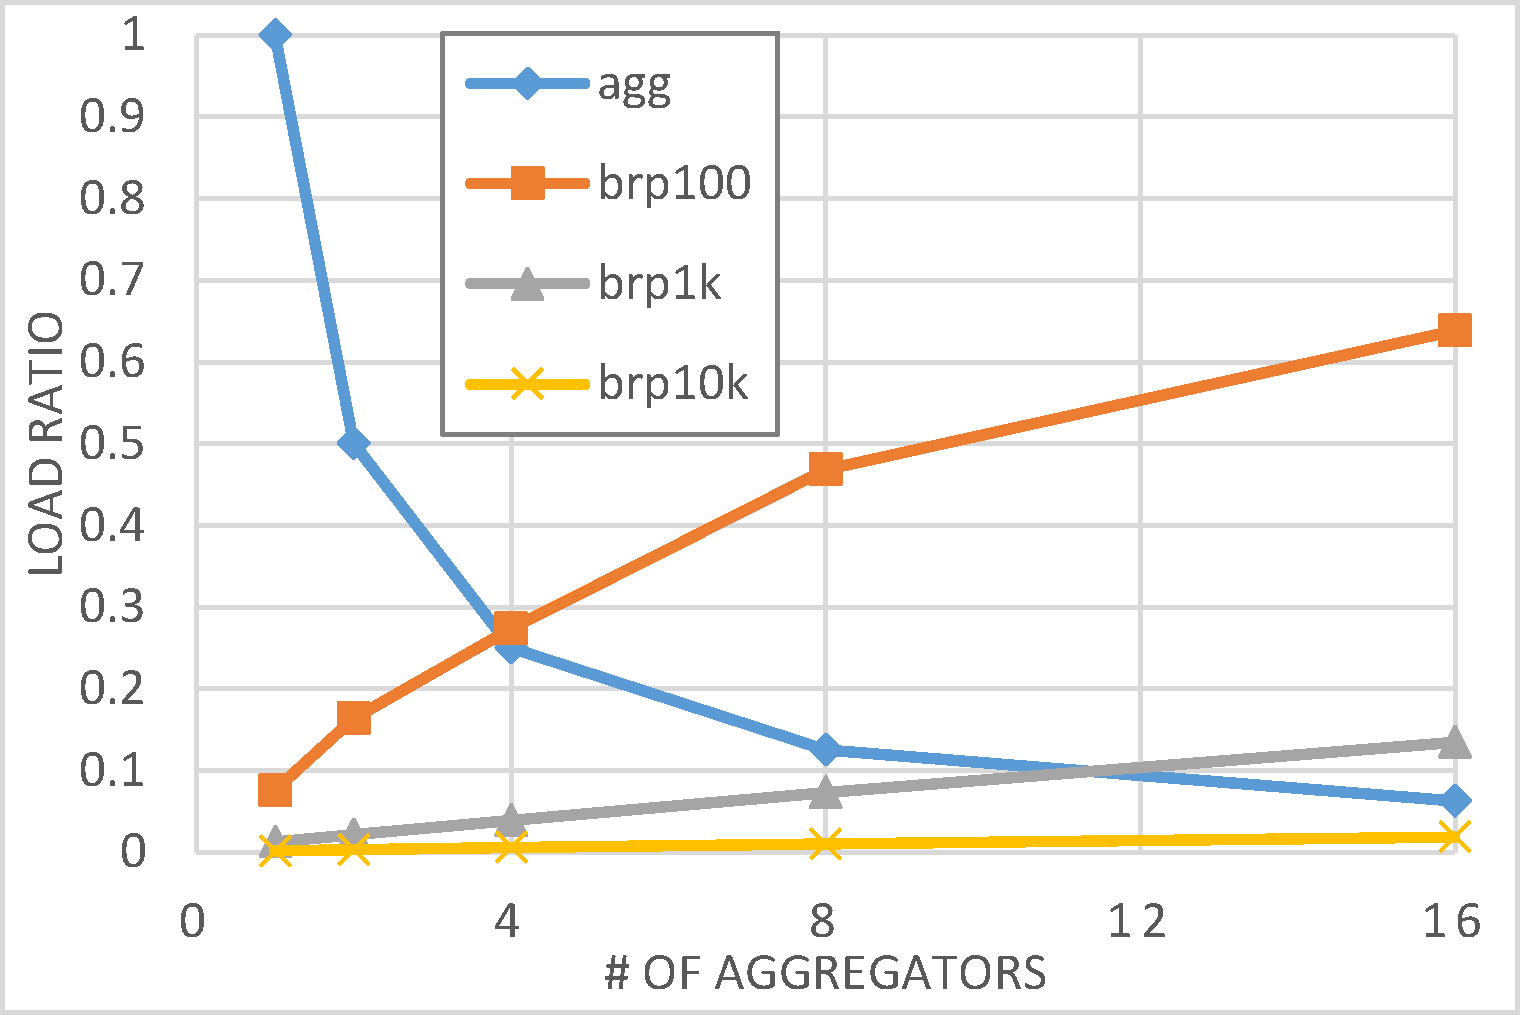
\includegraphics[width=0.75\columnwidth]{images/resultD.pdf}
\caption{The intersections with the blue line shows the optimal amount of aggregator nodes for a given amount of flex-offers send per time unit.}%
\label{fig:resultC}%
\end{figure}


In Figure \ref{fig:resultA} the load on the BRP node is shown in a double logarithmic graph. 
The legend shows the number of aggregator nodes corresponding to the six different strategies, 
the x-axis is the total number of flex-offers sent, 
and the y-axis shows the total number of flex-offers the BRP node receives, this is know as load.

In Figure \ref{fig:resultB} the load on the aggregator node\(s\) is shown. 
The x-axis is the total number of flex-offers sent, 
and the y-axis is the maximum load of the set of aggregator nodes used. 
Remember that all the strategies use round-robin algorithm as distribution function, thus, all the flex-offers is distributed almost evenly. 

The results indicate that load on the BRP node is lower if only one aggregator node is used. 
This is because when the flex-offers are spread across more aggregator nodes the aggregator node will not be able to aggregate as many flex-offers as if one single aggregator node had all the flex-offers. 
This means that if one aggregator node receive all the flex-offers then is able to reduce the number of flex-offers sent to the BRP node.

We assume that it is desirable that the number of flex-offers received by both the aggregator nodes and the BRP node is kept as low as possible.
It is possible to combine the two graphs and find the intersections.
The intersections represents the optimal number of aggregator nodes at the given number of flex-offers sent per time unit. 

In Figure \ref{fig:resultC} the load of the aggregator nodes and the load of the BRP node is displayed.
The x-axis is the number of aggregator nodes, and the y-axis is a percentage representation of the load on the nodes.
The blue line represents load on the aggregator node.
The red, grey, and blue are the load on the BRP node with respectively with an average of 100, 1000, and 10,000 flex-offers send per time unit.
%Beskriv dette mereget mere, resultater.

The two visible intersections indicate the optimal set of aggregator nodes at an given average of flex-offers sent. 
These results allows us to determine the number of aggregator nodes to use when the average number of flex-offers sent is know, and our proposed strategy is used.   

\section{Conclusion and future work}
By moving the aggregation functionality from the BRP node to a set of aggregation nodes, we have reduced the overall number of flex-offers sent to the BRP node.
We distribute the flex-offers to the aggregator nodes using round robin.   
The aggregator nodes sent the aggregated flex-offers to the BRP node.
A strategy can be defined to describe the configuration of this set-up.
Strategies can be compared with different parameters. 
For a given strategy is it possible, by varying the number of aggregator nodes, to find an optimal number of aggregator nodes for a given average of flex-offers sent.


In a real world scenario the number of flex-offers sent may vary great during the course of a whole day. 
This implies the need of adjusting the number of aggregator nodes used, this is only the case if Evenly Distribution Strategy is used.
For further work more advanced strategies can be developed where the distribution strategy distributes based on how the aggregation strategy. 
This would course the aggregation to be better but might also result in uneven load on the aggregator nodes.  

%Skriv mere om hvor lidt data vi har.


\appendix
\bibliography{bibtex/bib}{}

\end{document}